\documentclass[tikz,border=10pt]{standalone}
\usepackage{tikz}
\usepackage{amsmath}
\usetikzlibrary{arrows.meta, positioning, calc, shapes.geometric, backgrounds}

% Define colors
\definecolor{emeraldpine}{HTML}{1A4D3E}
\definecolor{harvardcrimson}{HTML}{A51C30}
\definecolor{ethdarkblue}{HTML}{1F407A}
\definecolor{ethpetrol}{HTML}{007A87}
\definecolor{ethbronze}{HTML}{B87333}
\definecolor{ethpurple}{HTML}{5B4B8A}
\definecolor{ink}{HTML}{1A202C}
\definecolor{softink}{HTML}{4A5568}
\definecolor{paleink}{HTML}{A0AEC0}
\definecolor{cardbg}{HTML}{F8FAFC}
\definecolor{shadecolor}{HTML}{F4F6F9}
\definecolor{safegreen}{HTML}{059669}

\begin{document}
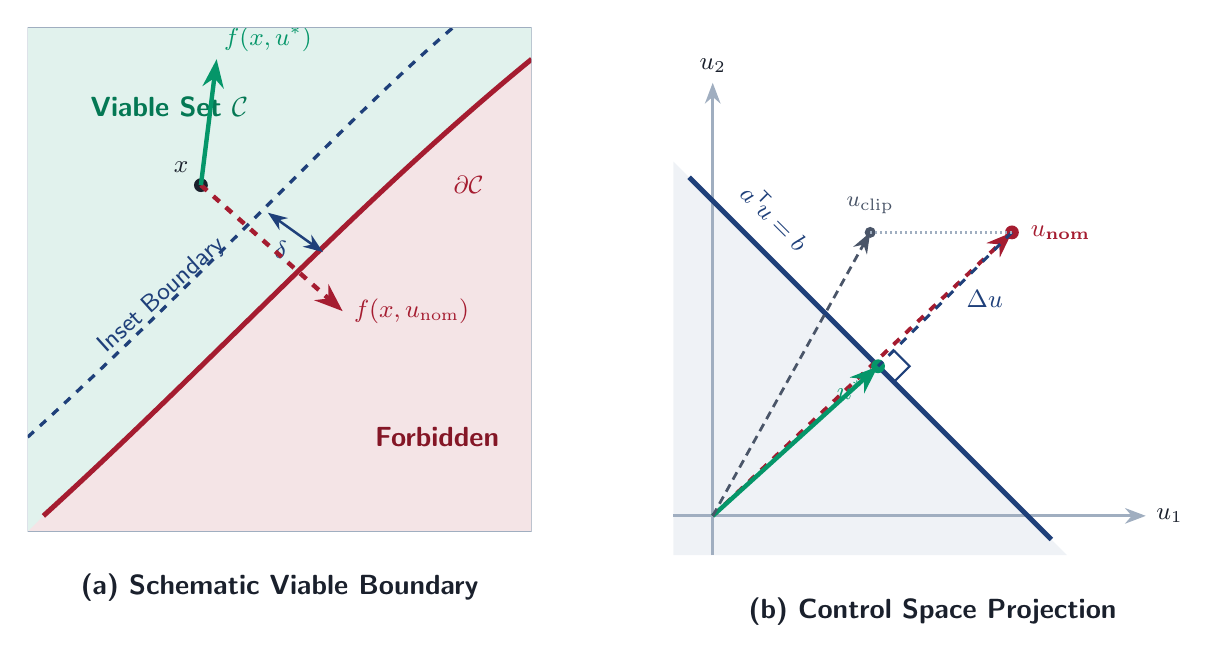
\begin{tikzpicture}[
    font=\sffamily,
    >=Stealth,
    line width=1pt
]

% ===== Panel (a): State space =====
\begin{scope}[local bounding box=panela]
    \clip (-0.2,-0.2) rectangle (6.2,6.2);

    % Safe region fill
    \fill[safegreen!12] (-0.2,-0.2) rectangle (6.2,6.2);

    % Forbidden region fill (below/right of the curved boundary)
    \fill[harvardcrimson!12]
        (0, 0) .. controls (2.2, 2.0) and (4.0, 4.0) .. (6.2, 5.8)
        -- (6.2,-0.2) -- (-0.2,-0.2) -- cycle;

    % Physical boundary ∂C (solid red curve)
    \draw[harvardcrimson, line width=1.8pt]
        (0, 0) .. controls (2.2, 2.0) and (4.0, 4.0) .. (6.2, 5.8);
    \node[harvardcrimson, font=\sffamily\bfseries\small] at (5.4, 4.2) {$\partial\mathcal{C}$};

    % Inset boundary (dashed blue, shifted inward)
    \draw[ethdarkblue, dashed, line width=1.2pt]
        (-0.2, 1.0) .. controls (2.0, 3.0) and (3.8, 5.0) .. (5.2, 6.2);
    \node[ethdarkblue, font=\sffamily\small, rotate=42] at (1.5, 2.8) {Inset Boundary};

    % Margin δ indicator between curves
    \draw[<->, ethdarkblue, line width=0.9pt] (3.55, 3.35) -- (2.85, 3.85)
        node[midway, below left=-1pt, font=\small] {$\delta$};

    % Set labels
    \node[safegreen!80!black, font=\sffamily\bfseries] at (1.6, 5.2) {Viable Set $\mathcal{C}$};
    \node[harvardcrimson!80!black, font=\sffamily\bfseries] at (5.0, 1.0) {Forbidden};

    % State point x
    \coordinate (x) at (2.0, 4.2);
    \fill[ink] (x) circle (2.5pt);
    \node[ink, above left=1pt, font=\small] at (x) {$x$};

    % Unsafe nominal vector f(x, u_nom) — heading toward boundary
    \draw[->, harvardcrimson, dashed, line width=1.6pt]
        (x) -- ++(1.8, -1.6) node[right, font=\small] {$f(x, u_{\text{nom}})$};

    % Safe corrected vector f(x, u*) — tangent/away from boundary
    \draw[->, safegreen, line width=1.6pt]
        (x) -- ++(0.2, 1.6) node[above right=-2pt, font=\small] {$f(x, u^*)$};

    % Bounding box
    \draw[paleink, line width=0.5pt] (-0.2,-0.2) rectangle (6.2,6.2);
\end{scope}

\node[below=0.4cm of panela, font=\sffamily\bfseries, ink] {(a) Schematic Viable Boundary};

% ===== Panel (b): Control space =====
\begin{scope}[xshift=8.5cm, local bounding box=panelb]
    % Admissible half-space fill: u1 + u2 <= 4 (below the line)
    \fill[ethdarkblue!7] (-0.5,-0.5) -- (-0.5, 4.5) -- (4.5, -0.5) -- cycle;

    % Axes
    \draw[->, paleink, line width=1pt] (-0.5, 0) -- (5.5, 0) node[right, ink, font=\small] {$u_1$};
    \draw[->, paleink, line width=1pt] (0, -0.5) -- (0, 5.5) node[above, ink, font=\small] {$u_2$};

    % Constraint hyperplane: u1 + u2 = 4 (slope = -1)
    \draw[ethdarkblue, line width=1.8pt] (-0.3, 4.3) -- (4.3, -0.3);
    \node[ethdarkblue, font=\sffamily\bfseries\small, rotate=-45] at (0.8, 3.8) {$a^\mathsf{T}\! u = b$};

    % Admissible half-space is conveyed by the blue shading

    % Origin
    \coordinate (O) at (0,0);

    % u_nom — outside safe half-space (upper right, clearly infeasible)
    \coordinate (unom) at (3.8, 3.6);
    \draw[->, harvardcrimson, dashed, line width=1.4pt] (O) -- (unom);
    \fill[harvardcrimson] (unom) circle (2.5pt);
    \node[harvardcrimson, right=3pt, font=\small\bfseries] at (unom) {$u_{\text{nom}}$};

    % u* — orthogonal projection of u_nom onto constraint line u1+u2=4
    % Projection of (3.8,3.6) onto u1+u2=4: midpoint = (2.0, 2.0)
    \coordinate (ustar) at (2.1, 1.9);
    \draw[->, safegreen, line width=1.6pt] (O) -- (ustar);
    \fill[safegreen] (ustar) circle (2.5pt);
    \node[safegreen, below left=2pt, font=\small\bfseries] at (ustar) {$u^*$};

    % Projection line Δu from u_nom to u* (perpendicular to constraint)
    \draw[ethdarkblue, dashed, line width=1.1pt] (unom) -- (ustar);
    \node[ethdarkblue, font=\small, right=4pt] at ($(unom)!0.5!(ustar)$) {$\Delta u$};

    % Right-angle mark at u* (perpendicular to constraint line)
    % Constraint line direction: (1,-1)/sqrt(2); perpendicular: (1,1)/sqrt(2)
    \coordinate (perp1) at ($(ustar) + (0.2, -0.2)$);   % along constraint
    \coordinate (perp2) at ($(perp1) + (0.2, 0.2)$);     % perpendicular corner
    \coordinate (perp3) at ($(ustar) + (0.2, 0.2)$);     % toward u_nom
    \draw[ethdarkblue, line width=0.8pt] (perp1) -- (perp2) -- (perp3);

    % u_clip — per-axis component clamping (clamp u1 to feasible, keep u2)
    % If u_nom=(3.8,3.6), naively clamping u1 to fit: u_clip ≈ (0.4, 3.6)
    % This shows component-wise clamping gives wrong direction
    \coordinate (uclip) at (2.0, 3.6);
    \draw[->, softink, densely dashed, line width=1pt] (O) -- (uclip);
    \fill[softink] (uclip) circle (2pt);
    \node[softink, above=3pt, font=\footnotesize] at (uclip) {$u_{\text{clip}}$};

    % Guide lines showing per-axis clamping from u_nom
    \draw[paleink, densely dotted, line width=0.8pt] (unom) -- (uclip);

\end{scope}

\node[below=0.4cm of panelb, font=\sffamily\bfseries, ink] {(b) Control Space Projection};

\end{tikzpicture}
\end{document}
